\documentclass{article}

\RequirePackage{luatex85}
\usepackage{fontspec}
\usepackage[all]{xy}

\usepackage{fancyhdr}
\usepackage{extramarks}
\usepackage{amsthm,amsmath,amssymb,physics}
\usepackage{tikz}
\usepackage{float}
\usepackage{subcaption}
\usepackage{graphicx}
\usepackage{siunitx}

% ====================
% Basic Document Settings
%

\topmargin=-0.45in
\evensidemargin=0in
\oddsidemargin=0in
\textwidth=6.5in
\textheight=9.0in
\headsep=0.25in

\linespread{1.1}

\pagestyle{fancy}
\lhead{\hmwkAuthorName}
\chead{\hmwkClass : \hmwkTitle}
\rhead{\firstxmark}
\lfoot{\lastxmark}
\cfoot{\thepage}

\renewcommand\headrulewidth{0.4pt}
\renewcommand\footrulewidth{0.4pt}

\setlength\parindent{0pt}

%
% Create Problem Sections
%

\newcommand{\enterProblemHeader}[1]{
    \nobreak\extramarks{}{Problem \arabic{#1} continued on next page\ldots}\nobreak{}
    \nobreak\extramarks{Problem \arabic{#1} (continued)}{Problem \arabic{#1} continued on next page\ldots}\nobreak{}
}

\newcommand{\exitProblemHeader}[1]{
    \nobreak\extramarks{Problem \arabic{#1} (continued)}{Problem \arabic{#1} continued on next page\ldots}\nobreak{}
    \stepcounter{#1}
    \nobreak\extramarks{Problem \arabic{#1}}{}\nobreak{}
}

\setcounter{secnumdepth}{0}
\newcounter{partCounter}
\newcounter{homeworkProblemCounter}
\setcounter{homeworkProblemCounter}{1}
\nobreak\extramarks{Problem \arabic{homeworkProblemCounter}}{}\nobreak{}

%
% Homework Problem Environment
%
% This environment takes an optional argument. When given, it will adjust the
% problem counter. This is useful for when the problems given for your
% assignment aren't sequential. See the last 3 problems of this template for an
% example.
%
\newenvironment{homeworkProblem}[1][-1]{
    \ifnum#1>0
        \setcounter{homeworkProblemCounter}{#1}
    \fi
    \section{Problem \arabic{homeworkProblemCounter}}
    \setcounter{partCounter}{1}
    \enterProblemHeader{homeworkProblemCounter}
}{
    \exitProblemHeader{homeworkProblemCounter}
}

%
% Homework Details
%   - Title
%   - Due date
%   - Class
%   - Section/Time
%   - Instructor
%   - Author
%

\newcommand{\hmwkTitle}{Homework\ \#3}
\newcommand{\hmwkDueDate}{April 22, 2020}
\newcommand{\hmwkClass}{CS364/AM792}
\newcommand{\hmwkAuthorName}{\textbf{Unathi K. Skosana}}

%
% Title Page
%

\title{
    \vspace{2in}
    \textmd{\textbf{\hmwkClass:\ \hmwkTitle}}\\
    \normalsize\vspace{0.1in}\small{Due\ on\ \hmwkDueDate\ at 17:00pm}\\
    \vspace{3in}
}

\author{\hmwkAuthorName}
\date{}

\renewcommand{\part}[1]{\textbf{\large Part \Alph{partCounter}}\stepcounter{partCounter}\\}

%
% Various Helper Commands
%

% Alias for the Solution section header
\newcommand{\solution}{\textbf{\large Solution}}

\begin{document}

\maketitle

\pagebreak

\begin{homeworkProblem}
    \textbf{(a)}
    \\
    \\
    The points identified here for correspondence were along each of the axes,
    this was done to simply matters.

    \begin{figure}[H]
        \centering
        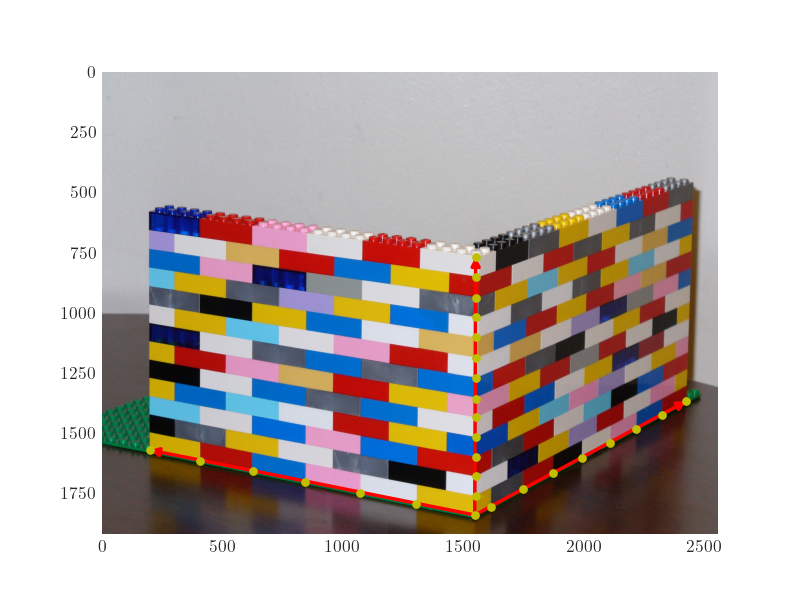
\includegraphics[height=3.5in]{./images/axis_lego1.png}
        \caption{Selected points for lego1.jpg}
    \end{figure}

    Using the known Lego dimensions (width, height, breadth) in millimetres, we
    can then find the corresponding points in the 3-space world coordinate system.

    \begin{figure}[H]
        \centering
        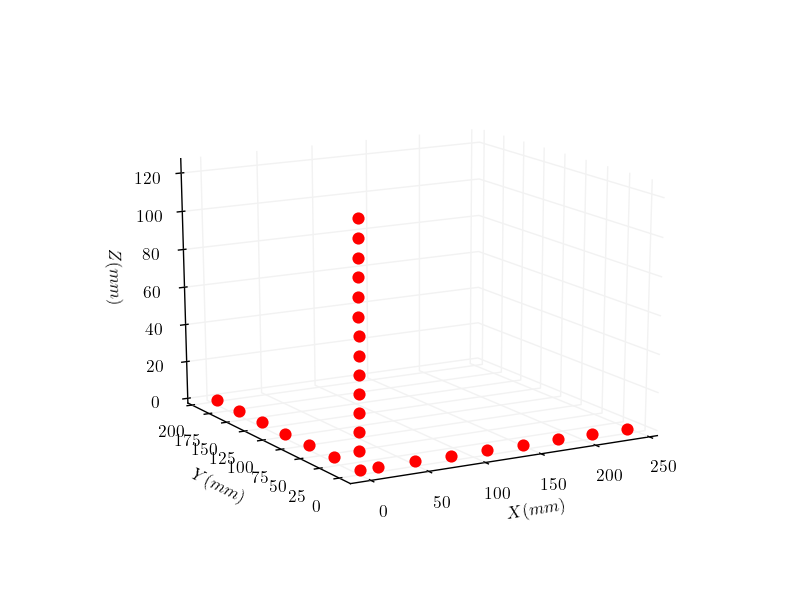
\includegraphics[width=0.65\linewidth]{./images/axis_lego1_3d.png}
        \caption{World coordinate system}
    \end{figure}

    The camera matrix $P$ was found to be

    \begin{align}
        P = \mqty[2.214\mathrm{e-}3 & -2.887\mathrm{e-}3 & -1.414\mathrm{e-}4
                                     & 6.440\mathrm{e-}1 \\
        -4.257\mathrm{e-}4 & -2.818\mathrm{e-}4 & -3.653\mathrm{e-}3
                           & 7.650\mathrm{e-}1 \\ 2.854\mathrm{e-}7 &
        1.920\mathrm{-e}7 & -9.732\mathrm{e-}8 &
                            4.154\mathrm{e-}4]
    \end{align} \\

    \textbf{(b)}
    \\
    \\

    (i)
    \\
    \\
    To prove that the $R=W\hat{Q}^\mathsf{T}$ is orthogonal, we show that
    $RR^\mathsf{T} = I$ 

    \begin{align*}
        RR^\mathsf{T} &= W\hat{Q}^\mathsf{T}(W\hat{Q}^\mathsf{T})^\mathsf{T} \\
                      &= W\hat{Q}^\mathsf{T}(\hat{Q}^\mathsf{T})^{\mathsf{T}}W^\mathsf{T} \\ 
                      &= W\hat{Q}^\mathsf{T}\hat{Q}W^\mathsf{T} \\
                      &= WIW^\mathsf{T}  \qquad &\text{ By definition from }
                  \hat{Q}\hat{R}\text{-decomposition } \hat{Q} \text{ is orthogonal } \\
                      &= I \qquad &\text{W orthogonal and real symmetric}
    \end{align*} \\

    \pagebreak

    (ii)
    \\
    \\
    By definition the matrix $\hat{R}$ is upper triangular, thus
    $\hat{R}^\mathsf{T}$ is lower triangular. Thus

    \begin{align*}
        W\hat{R}^\mathsf{T}W &= \mqty[0 & 0 & 1 \\ 0 & 1 & 0 \\ 1 & 0 & 0]
        \mqty[a & 0 & 0 \\ b & c & 0 \\ d & e & f]\mqty[0 & 0 & 1 \\ 0 & 1 & 0 \\
        1 & 0 & 0]  \\
          &= \mqty[d & e & f \\ b & c & 0 \\ a & 0 & 0]\mqty[0 & 0 & 1 \\ 0 & 1 & 0 \\
        1 & 0 & 0] \\
        K &= \mqty[d & e & f \\ 0 & c & b \\ 0 & 0 & a]
    \end{align*}

    (iii)
    \\
    \\
    We can now prove that $KR[\mathbb{I}\text{ } | \text{ } \tilde{\mathbf{C}}]
    = P$

    \begin{align*}
        KR [\mathbb{I} \text{ } | \text{} -\tilde{\mathbf{C}}] &= W
        \hat{R}^\mathsf{T} W W \hat{Q}^\mathsf{T} [\mathbb{I}\text{ } |
        -\tilde{\mathbf{C}}]  \\
         &=W\hat{R}^\mathsf{T}\hat{Q}^\mathsf{T} [\mathbb{I}\text{ } |
        -\tilde{\mathbf{C}}] \\
         &= W(\hat{Q}\hat{R})^\mathsf{T} [\mathbb{I} | -\tilde{\mathbf{C}}]  \\
         &= WWP_{1:3} [\mathbb{I} | -\tilde{\mathbf{C}}] \\
         &= P_{1:3}[\mathbb{I} | (P_{1:3})^{-1}\mathbf{p}_4] \\
         &= [P_{1:3} | \mathbf{p}_4] \\
         &= P
    \end{align*}

    \pagebreak

    \textbf{(c)}
    \\
    \\

    \begin{align*}
            K &= \mqty[1.016\mathrm{e+}3 & 1.980\mathrm{e+}2 & 7.159\mathrm{e+}2  \\
            0.0              & 1.022\mathrm{e+}4 & 1.408\mathrm{e+}3 \\
            0.0              & 0.0 & 1.0] \\
            R &= \mqty[0.558 & -0.830 & -0.001 \\
            -0.226 & -0.151 & -0.962 \\
            0.798 & 0.537 & -0.272] \\
            \tilde{\mathbf{C}} &= \mqty[-969.264 \\ -538.031 \\ 363.866]
    \end{align*}

\end{homeworkProblem}

\pagebreak

\begin{homeworkProblem}
    \textbf{(a)}
    \\
    \\
    Repeating problems 1a and 1c for the second Lego image. We get the
    $P$ and its decomposition

    \begin{align*}
        P &= \mqty[-3.450\mathrm{e-}3 & 1.850\mathrm{e-}3 & 9.524\mathrm{e-}5 &
            -4.874\mathrm{e-}1 \\
            2.309\mathrm{e-}4 & 4.227\mathrm{e-}4 & 3.957\mathrm{e-}3 &
            -8.731\mathrm{e-}1 \\
            -2.105\mathrm{e-}7 & -2.920\mathrm{e-}7 & 1.186\mathrm{e-}7 & -4.924\mathrm{e-}4
            ] \\ 
        K &= \mqty[1.024\mathrm{e+}4 & -3.083\mathrm{e+}1 & 1.373\mathrm{e+}3 \\
        0.0 & 1.031\mathrm{e+}4 & 2.069\mathrm{e+}3 \\ 
        0.0 & 0.0 & 1.0] \\
        R &= \mqty[-0.814 & 0.581 & -0.0146 \\
        0.171 & 0.263 & 0.950 \\ 
        -0.555 & -0.770 & 0.312] \\
        \tilde{\mathbf{C}} &= \mqty[-688.360 \\ -1039.170 \\ 371.833]
    \end{align*}

    The selected points are shown on the figure below

    \begin{figure}[H]
        \centering
        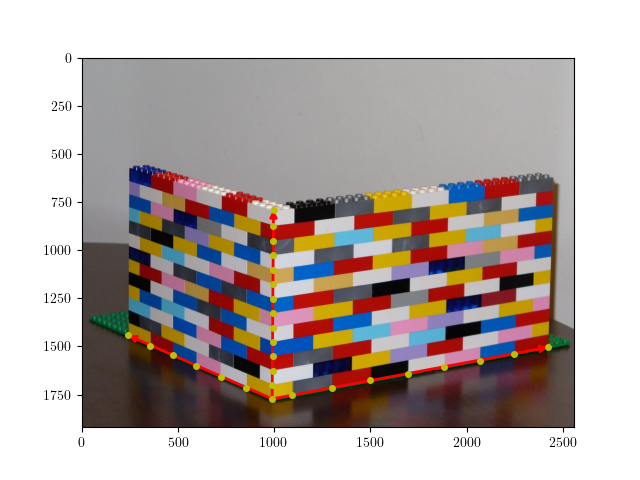
\includegraphics[height=3.5in]{./images/axis_lego2.png}
        \caption{Selected points for lego2.jpg}
    \end{figure} \\

    \pagebreak

    \textbf{(b)}
    \\
    \\
    Calculating the distances between the camera centres is as simple as
    calculating the norm of the difference vector between camera centres.

    \begin{align*}
        \left\Vert\tilde{\mathbf{C}_1}  - \tilde{\mathbf{C}_2}\right\Vert = 574.552
        \si{\milli\metre}
    \end{align*}

    The principal axis is the $z$-axis of the camera. This axis is perpendicular
    to the principal plane of the image. The points on this plane
    map to a line at infinity of the image, meaning that for some $\mathbf{X}$ in 3-space

    \begin{align*}
        P\mathbf{X} = (x,y,0)^{T} \implies P_3^{T}\mathbf{X} = 0
    \end{align*}
    where $\mathbf{P}_3^{T}$ is the third row of $P$. \\

    Since a vector $\mathbf{v} = (p_{31}, p_{32}, p_{33})^{T}$ is perpendicular to the plane
    $P_3^\mathsf{T} = (p_{31}, p_{32}, p_{33}, p_{34})$. Thus the principal
    axis vector is given by $\mathbf{v}$ and it can be extracted from the last row of $KR$. However, due to fact that $P$ is
    defined up to a sign there is ambiguity whether $-\mathbf{v}$  or
    $-\mathbf{v}$ points towards or from the camera centre. The ambiguity is
    resolved assigning $\mathbf{v'} = \mathrm{det}(KR)\mathbf{v}$ as principal
    axis vector, which always points towards the camera centre irregardless of the
    scaling of $P$. \\

    We can thus find the angle between the principal axes of the two cameras
    through

    \begin{align}
        \theta = \mathrm{arcos}\left(\frac{\mathbf{v_1'} \cdot \mathbf{v_2'}}{
    ||\mathbf{v_1'}|| \cdot ||\mathbf{v_2'}||}\right) = \ang{19.545}
    \end{align} \\

    \textbf{(c)}
    \\
    \\
    Following the logic as in the previous question, the first and second of
    $KR$ give the direction vectors for the $x$-axis and $y$-axis respectively.
    We can thus use these to plot the camera axes. Below are different views of
    the 2-camera system in world coordinates.

    \begin{figure}[H]
        \centering
        \begin{subfigure}{0.49\textwidth}
            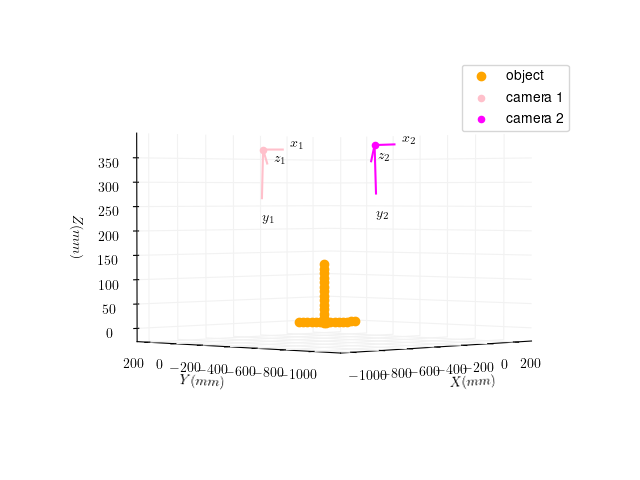
\includegraphics[width=0.9\linewidth]{images/ang_1.png}
        \end{subfigure}
        \begin{subfigure}{0.49\textwidth}
            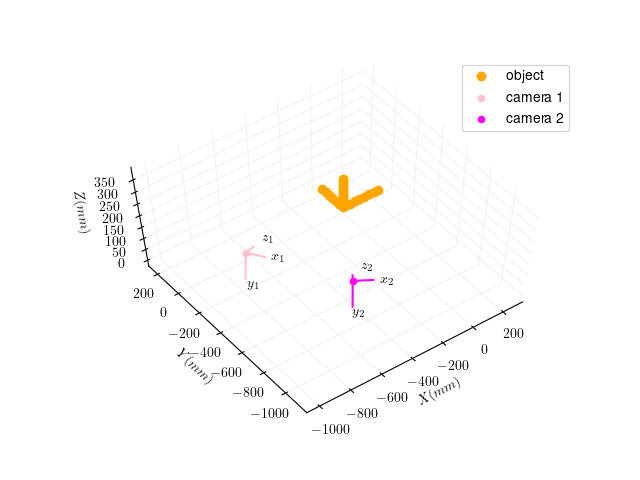
\includegraphics[width=0.9\linewidth]{images/ang_2.png}
        \end{subfigure}
    \end{figure}
    \begin{figure}[H]
        \begin{subfigure}{0.49\textwidth}
            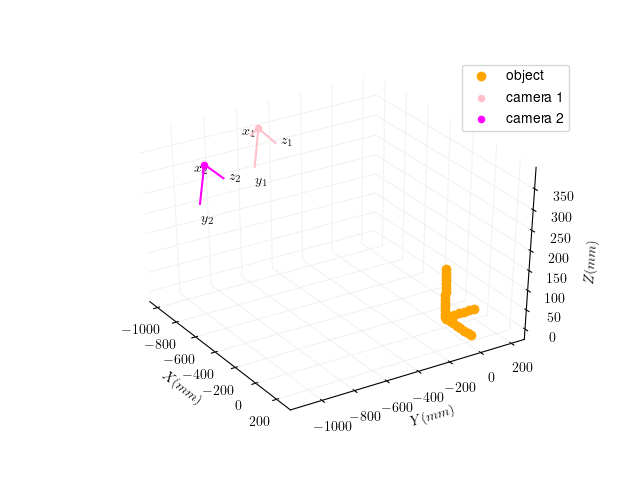
\includegraphics[width=0.9\linewidth]{images/ang_3.png}
        \end{subfigure}
        \begin{subfigure}{0.49\textwidth}
            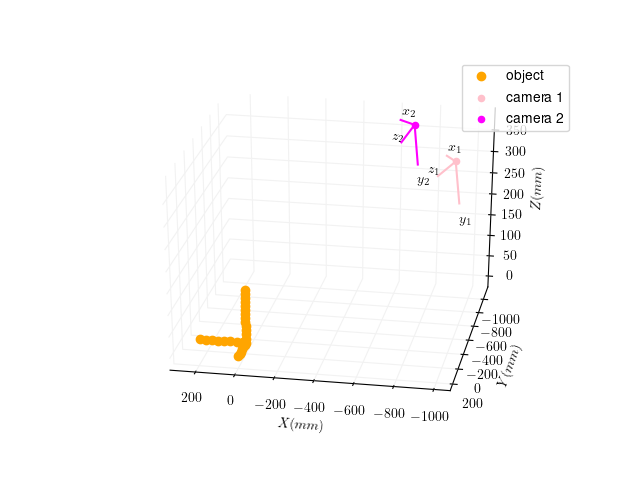
\includegraphics[width=0.9\linewidth]{./images/ang_4.png}
        \end{subfigure}
        \begin{subfigure}{0.49\textwidth}
            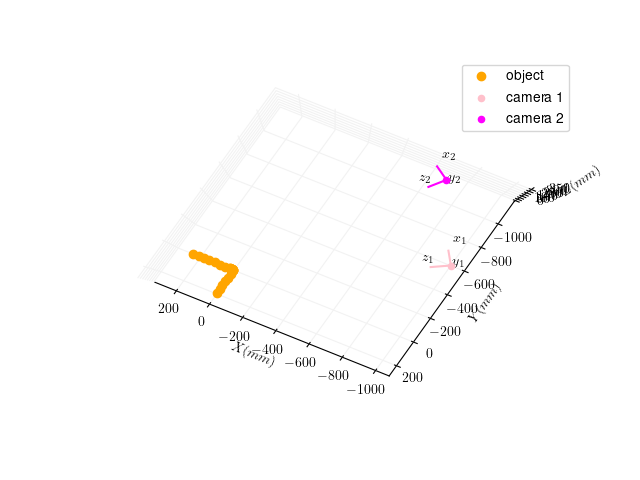
\includegraphics[width=0.9\linewidth]{./images/ang_5.png}
        \end{subfigure}
        \begin{subfigure}{0.49\textwidth}
            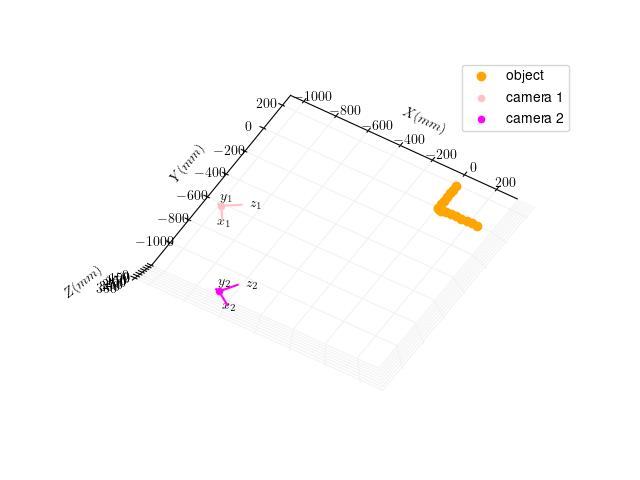
\includegraphics[width=0.9\linewidth]{./images/ang_6.png}
        \end{subfigure}
        \caption{Different views of the camera axes in the world coordinate system}
    \end{figure}
\end{homeworkProblem}

\pagebreak

\begin{homeworkProblem}
    Let $\mathbf{D}_i$ be a 4-vector with the entry $1$ at index $i$ and $0$ entries
    everywhere else (direction vectors of each the axes). i.e $\mathbf{D}_1 = (1, 0, 0, 0)^\mathsf{T}$. Then

    \begin{align}
        P\mathbf{D}_i = [\mathbf{p}_1\text{ }\mathbf{p}_2\text{
        }\mathbf{p}_3\text{ }\mathbf{p}_4]\mathbf{D}_i = \mathbf{p}_i
    \end{align}

    Thus the directional vectors of each axes in the world coordinate frame are
    projected onto the points (after being de-homogenized) $\mathbf{p}_i$ on the image and $\mathbf{D}_4$ is
    the world origin and $\mathbf{p}_4$ will be projection of the world origin
    on the image. Performing the projections as describe, we can image the world axes on the
    image and draw them. One small issue encountered was that the projections
    of directional axis vectors produced imaged points that fell outside the
    image range. This was circumvented by appropriately scaling them to
    produce the images below. \\

    \begin{figure}[H]
        \centering
        \begin{subfigure}{.6\textwidth}
            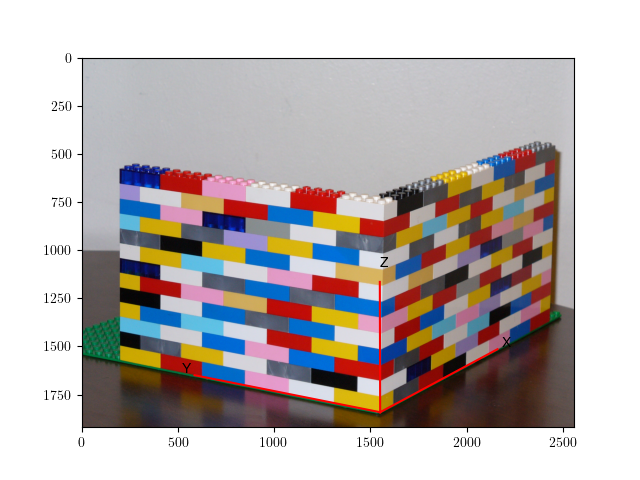
\includegraphics[width=0.9\linewidth]{./images/imaged_axis_lego1.png}
        \end{subfigure}

        \begin{subfigure}{.6\textwidth}
            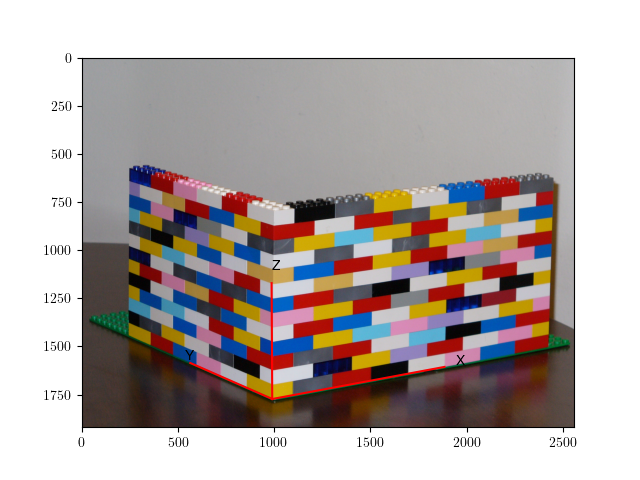
\includegraphics[width=0.9\linewidth]{./images/imaged_axis_lego2.png}
        \end{subfigure}
    \end{figure}

\end{homeworkProblem}

\pagebreak

\begin{homeworkProblem}
    \textbf{(a)}
    \\
    \\
    Computing the epipoles as described gives

    \begin{align*}
        \mathbf{e} &= (-1.231\mathrm{e+}5,  4.453\mathrm{e+}2)^\mathsf{T} \\
        \mathbf{e'}  &= (-2.150\mathrm{e+}4, -1.310\mathrm{e+}3)^\mathsf{T}
    \end{align*}

    Both the epipoles fall outside their respective image ranges. However, this
    does indeed make sense since the each of the cameras are not in each other's
    "views". In world coordinate system, the camera are roughly at the same height
    and one is to the side of the other. \\

    \textbf{(b)}
    \\
    \\
    From $P', P, e'$, the Fundamental matrix can be computed as

    \begin{align*}
        F = \mathbf{e'} \times P' P^\mathsf{T} (PP^\mathsf{T})^{-1}
    \end{align*}

    doing so, gives

    \begin{align*}
        F &= \mqty[-1.516\mathrm{e-}6 & -9.533\mathrm{e-}5 & -1.441\mathrm{e-}1 \\
        1.884\mathrm{e}-5 & 1.320\mathrm{e-}6 & 2.319\mathrm{e+}0 \\
        -7.930\mathrm{e-}3 & -2.0479\mathrm{e+}0 & -6.442\mathrm{e+}1]
    \end{align*} \\

    \textbf{(c)}
    \\
    \\
    In order to find the epipolar lines, we first have find matches between the
    two images. In this case we can manually select the matches. Then for a
    match $\mathbf{x}_1$ on image 1 we determine the epipolar line $F\mathbf{x}
    = \mathbf{\ell}'_1 = (a, b, c)^\mathsf{T}$ on image 2. To draw the line,
    we solve the equation

    \begin{align*}
        ax + by + c = 0 \implies y = - \frac{ax + c}{b}
    \end{align*}

    where $x$ goes over the width of image 2. The procedure is similar for
    epipolar lines on image 1. Following this procedure, Fig.~\ref{fig:epipolars} was
    produced. The epipolar lines don't perfectly go through their corresponding matches
    due to some errors in the manual match-selecting.


    \begin{figure}[H]
        \centering
        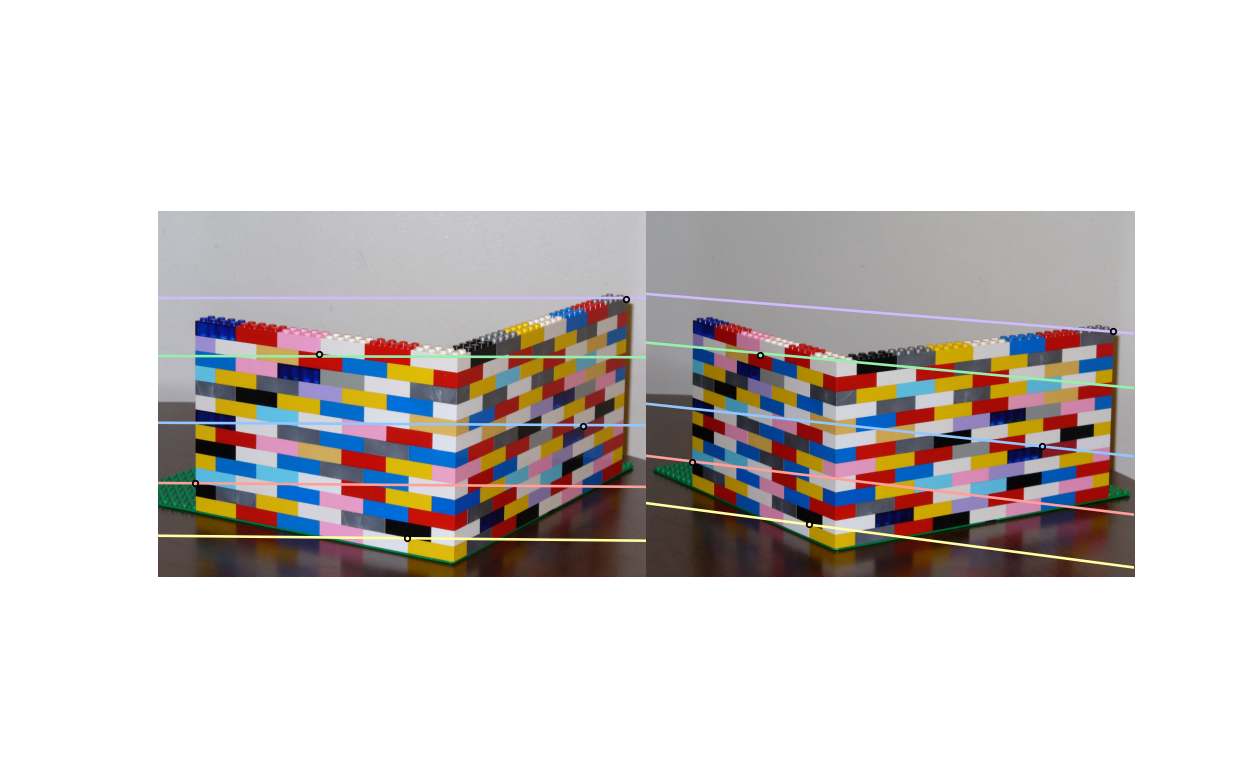
\includegraphics[width=0.95\linewidth]{./images/epipolar_lines.png}
        \caption{Epipolar lines for corresponding points across the two image
        planes.}
        \label{fig:epipolars}
    \end{figure}

\end{homeworkProblem}

\section{References}
Hartley, R., Zisserman, A. (2003). Multiple View Geometry in Computer Vision. New York, NY, USA: Cambridge University Press. ISBN: 0521540518



\end{document}
